

\chapter{Kostenanalyse und Vergleich zu anderen Deckensystemen}
Durch eine Analyse der Material und Herstellkosten soll eine Einordnung in den Markt untersucht werden.\\
\cite{1}
Die Basis für die Abmessungen des Sandwichträgers war der Bauteil-Versuchsköper mit einer Spannweite von l = \unit[7,20]{m}. Die Breite der Platte ($b=\unit[2,40]{m}$) wurde im Hinblick auf die zulässige Transportbreite gewählt.
Für den folgenden Kostenvergleich wurden Deckensysteme gewählt, die für diese Spannweite im Büro- und Industriebau üblicherweise eingesetzt werden (Ortbeton, Elementdecke, Hohldielendecke) oder in Zukunft verstärkt zur Anwendung kommen (Holz-Beton-Verbund, BSP). 
Der erste Aspekt sind die Materialkosten, die über übliche Marktpreise inklusive geschätzter Nachlässe bei größeren Bauprojekten ermittelt wurden. %Die Transport- und Montagekosten sind durch das Gewicht und die Abmessungen der vorgefertigten Elemente (Bereitstellung eines Autokrans) und die zusätzlich notwendigen Arbeiten (Ausbildung eines Rosts, Aufbeton, Schalung, etc.) bestimmt.



\section{Ausgewählte Deckensysteme}
Bei der Auswahl der zu vergleichenden Systeme wurde auf folgendes geachtet:\\
\begin{itemize}
	\item Verfahren (Vorfertigung, vor Ort gefertigt)
	\item Materialauswahl (Holz, Beton)
%	\item Transport (Abmessungen, Gewicht)
\end{itemize}
Vergleichssysteme:\\

\begin{itemize}
\item Holz-Beton-Verbunddecke (vgl. http://www.hbv-tt.de/)
\item Holzmassivbau Brettsperrholz (BSP oder X-Lam)
\item Ortbetondecke
\item Elementdecke
\item Hohldielendecke
\end{itemize}

\section{Verwendete Materialien für den Sandwichaufbau}

\subsection{Beton}

\begin{figure}[h!]
\begin{tabular}{|c|c|}
\hline 
Beton & SVB \\ 
\hline \hline
Dichte & 2300\,$ kg/m^{2}$ \\ 
\hline 
Dicke & 6,0\, $cm$ \\ 
\hline 
Preis & 123\,/$m^{2}$ \\ 
\hline 
\end{tabular} 
\end{figure}


\subsection{Holzbeton}

\begin{figure}[h!]
\begin{tabular}{|c|c|c|}
\hline 
Holzbeton & Velox WSD 50 & Velolx WSD 75 \\ 
\hline \hline
Dichte & 750 $ kg/m^{2}$ &750 $ kg/m^{2}$ \\ 
\hline 
Dicke & 5,0 $cm$ & 7,5 $cm$\\ 
\hline 
Preis & 254\,\euro/$m^{2}$ & 239\,\euro/$m^{2}$ \\ 
\hline 
\end{tabular} 
\end{figure}

\subsection{Holz}

\begin{figure}[h!]
\begin{tabular}{|c|c|}
\hline 
Holz & BSP \\ 
\hline \hline
Dichte & 550 $ kg/m^{3}$  \\ 
\hline 
Dicke & 11,8 $cm$ \\ 
\hline 
Preis & 500\,\euro/$m^{3}$\\ 
\hline 
\end{tabular} 
\end{figure}

\subsection{Verbindungsmittel}





\begin{figure}[h!]
\begin{tabular}{|c|c|}
\hline 
Schrauben & WR-T\,9\,x\,400  \\ 
\hline \hline
Gewicht & 0,158 $ kg/Stk.$ \\ 
\hline 
Preis & 2,15\,\euro/Stk  \\ 
\hline 
\end{tabular} 
\end{figure}	

\begin{figure}[h!]
\begin{tabular}{|c|c|c|}
\hline 
Kleber & Sikadur 31 & Sikatop 109 \\ 
\hline \hline
Dichte & 1650 $ kg/m^{3}$& 2000 $ kg/m^{3}$\\ 
\hline
Bedarf/Fläche& 4,2 $kg/m^{2} $& 4,2 $kg/m^{2} $ \\
\hline 
Preis & 4,50\,\euro/$m^{2}$ & 2,00\,\euro/$m^{2}$  \\ 
\hline 
\end{tabular} 
\end{figure}

\newpage
\section{Sandwichbauteile: Holz-Holzspanbeton}

\subsection{Bauteil 1}
Der dargestellte Bauteil ist gleich dem ersten Bauteilversuch.
\begin{figure}[h!]
\begin{center}
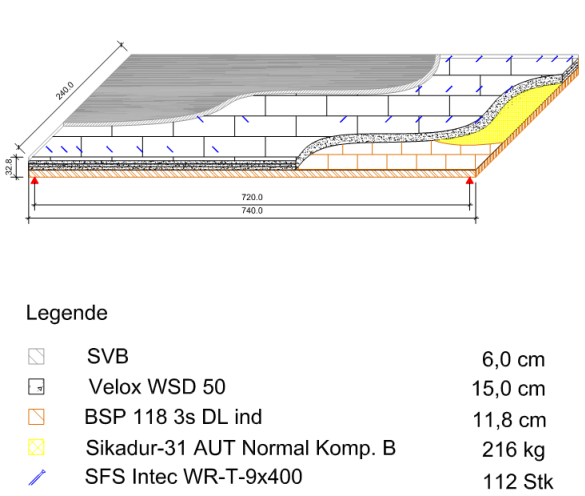
\includegraphics[scale =0.8]{Wirtschaftlichkeitsvergleich/Varianten/var1.jpg}
\caption{Aufbau der Sandwichplatte wie der Bauteil 1}
\end{center}
\end{figure}


\begin{figure}[h!]
\begin{center}
\begin{tabular}{|c|c|c|c|c|c|c|}
\hline 
Komponente & Bezeichnung & Volumen & Masse & Menge & Einheitspreis & Kosten \\ 

 &  & $m^{3}$ & kg &  &  & \euro \\ 
\hline \hline
Beton & SVB & 1,04 & 2385,0  & 1,04 $m^{3}$ & 123,0\,\euro / $m^{3}$ & 127,53 \\ 
\hline 
Holzlbeton & Velox WS 50 & 2,59 & 1944,0  & 2,59 $m^{3}$ & 264,0\,\euro / $m^{3}$ & 684,29 \\ 
\hline 
Holz & BSP 118 3s DL ind & 2,04 & 1121,0 & 2,04 $m^{3}$ & 500,0 \,\euro / $m^{3}$ & 1019,52 \\ 
\hline 
Schrauben & WR-T 9x400 & - & 17,7 & 122 $Stk.$ & 2,15 \,\euro / $Stk.$ & 240,80 \\ 
\hline 
Kleber & Sikadur 31  & - & 216  & 216 $kg$ & 4,5 \,\euro / $kg$& 972,00 \\ 
\hline \hline
Summe & &  & 5684 &  &  & 3044,13 \\ 
\hline 
Preis /$m^{2}$&  & &  &  &  & \textbf{176,17} \\ 
\hline 
\end{tabular} 
\end{center}
\end{figure}



\newpage
\subsection{Bauteil 3}
Der dargestellte Bauteil ist gleich dem ersten Bauteilversuch.
\begin{figure}[h!]
\begin{center}
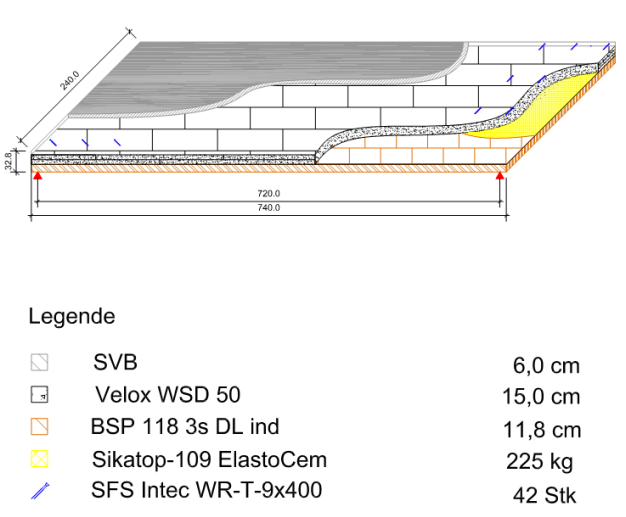
\includegraphics[scale =0.8]{Wirtschaftlichkeitsvergleich/Varianten/var3.jpg}
\caption{Aufbau der Sandwichplatte wie derBauteil 3}
\end{center}
\end{figure}

\begin{figure}[h!]
\begin{center}
\begin{tabular}{|c|c|c|c|c|c|c|}
\hline 
Komponente & Bezeichnung & Volumen & Masse & Menge & Einheitspreis & Kosten \\ 

 &  & $m^{3}$ & kg &  &  & \euro \\ 
\hline \hline
Beton & SVB & 1,04 & 2385,0  & 1,04 $m^{3}$ & 123,0\,\euro / $m^{3}$ & 127,53 \\ 
\hline 
Holzlbeton & Velox WS 50 & 2,59 & 1944,0  & 2,59 $m^{3}$ & 264,0\,\euro / $m^{3}$ & 684,29 \\ 
\hline 
Holz & BSP 118 3s DL ind & 2,04 & 1121,0 & 2,04 $m^{3}$ & 500,0 \,\euro / $m^{3}$ & 1019,52 \\ 
\hline 
Schrauben & WR-T 9x400 & - & 6,6 & 42 $Stk.$ & 2,15 \,\euro / $Stk.$ & 90,30 \\ 
\hline 
Kleber & SikaTop-109  & - & 225 & 225 $kg$ & 2,0 \,\euro / $kg$& 450,0 \\ 
\hline \hline
Summe & &  & 5682 &  &  & 2371,63 \\ 
\hline 
Preis /$m^{2}$&  & &  &  &  & \textbf{137,25} \\ 
\hline 
\end{tabular} 
\end{center}
\end{figure}










\newpage
\subsection{vorgeschlagener Bauteil}
Der dargestellte Bauteil ist gleich dem dritten Bauteilversuch mit 
\begin{figure}[h!]
\begin{center}
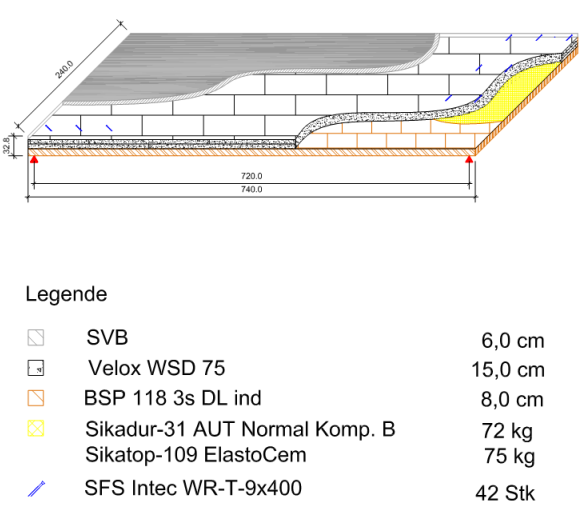
\includegraphics[scale =0.8]{Wirtschaftlichkeitsvergleich/Varianten/var_opti.jpg}
\caption{Aufbau der Sandwichplatte bei Optimierung des Bauteil 3}
\end{center}
\end{figure}


\begin{figure}[h!]
\begin{center}
\begin{tabular}{|c|c|c|c|c|c|c|}
\hline 
Komponente & Bezeichnung & Volumen & Masse & Menge & Einheitspreis & Kosten \\ 

 &  & $m^{3}$ & kg &  &  & \euro \\ 
\hline \hline
Beton & SVB & 1,04 & 2385,0  & 1,04 $m^{3}$ & 123,0\,\euro / $m^{3}$ & 127,53 \\ 
\hline 
Holzlbeton & Velox WS 75 & 2,59 & 1944,0  & 2,59 $m^{3}$ & 239,0\,\euro / $m^{3}$ & 619,49 \\ 
\hline 
Holz & BSP 118 3s DL ind & 2,04 & 1121,0 & 2,04 $m^{3}$ & 500,0 \,\euro / $m^{3}$ & 1019,52 \\ 
\hline 
Schrauben & WR-T 9x400 & - & 6,6 & 42 $Stk.$ & 2,15 \,\euro / $Stk.$ & 90,30 \\ 
\hline 
Kleber & SikaTop-109  & - & 75 & 75 $kg$ & 2,0 \,\euro / $kg$& 150,0 \\ 
Kleber & Sikadur 31  & - & 72  & 72 $kg$ & 4,5 \,\euro / $kg$& 324,0 \\ 
\hline \hline
Summe & &  & 5604 &  &  & 2330,83 \\ 
\hline 
Preis /$m^{2}$&  & &  &  &  & \textbf{134,89} \\ 
\hline 
\end{tabular} 
\end{center}
\end{figure}






\subsection{Abschätzung der  Arbeitszeit in der Produktion}

Die Annahmen für die Produktionszeit sind auf Grundlage der Bauteilversuche geschätzt worden.
Die Werte beziehen sich auf eine manuelle Fertigung, welche durch Einsatz von Maschinen verringert werden kann.


\begin{itemize}
\item Abmessungen 7,20\, x\, \unit[2,40]{m}
\item 3 Mann \'{a} \unit[30]{ \euro/h}
\end{itemize}

\begin{figure}[h!]
\begin{center}
\begin{tabular}{|c|c|c|c|}
\hline 
Tätigkeit & BT1 Arbeitszeit  & BT2 Arbeitszeit & BT3 Arbeitszeit\\ 
 & $[h]$  & $[h]$ & $[h]$\\ 
\hline \hline
Arbeitsvorbereitung & 0,50 & 0,50& 0,50 \\ 
\hline 
Verkleben der Holzbetonplatten & 1,50 & 1,50 & 1,0 \\ 
\hline 
Einbringen der Schrauben & 1,0& 0,5 & 0,5 \\ 
\hline 
Einschalen und Betonnieren & 1,0 & 1,0 & 1,0 \\ 
\hline \hline 
Summe $[h]$ & 4,0 & 3,50 & 3,0 \\ 
\hline
Preis/$m^{2}$ & 20,83 & 18,23 & 15,63 \\ 
\hline 
\end{tabular} 
\end{center}
\end{figure}


\subsection{Berechnung der Herstellkosten der Sandwichbauteile}

\begin{figure}[h!]
\begin{center}
\begin{tabular}{|c|c|c|c|}
\hline 
Bezeichnung & Materialpreis/\,$m^{2}$ & Arbeitskosten/\,$m^{2}$ & Herstellkosten/\,$m^{2}$ \\ 
\hline\hline 
Bauteil 1 & 176,17 & 20,83 & 197,00 \\ 
\hline 
Bauteil 3 & 137,25 & 18,23 & 155,48 \\ 
\hline 
vorgeschlagener Bauteil & 134,89 & 15,63 & 150,52 \\ 
\hline 
\end{tabular} 
\end{center}
\end{figure}






Die Differenz zwischen den BT1 und BT3 erklät sich aus der Reduktion der Anzahl der Schrauben und der Verwendung eines günstigeren Klebers. Die weitere Reduktion auf das optimierte Sandwichbauteil ist durch die Verwendung der dickeren Veloxplatten  und der geringeren Klebeschichten zurückzuführen. 


\section{Kostenvergleich mit anderen Deckensystemen}

Die Einheitspreise für die Produkte und Vergleichssysteme wurden durch Anfragen an Industriebetriebe, Bauunternehmen und Ingenieurbüros ermittelt. Die Vorgabe unsererseits waren: die Abmessungen wie in der Einleitung beschrieben und die Anwendung im Büro- und mehrgeschossigen Wohnbau.

\begin{figure}[h!]
\begin{center}
\begin{tabular}{|c|c|c|}
\hline 
Bezeichnung & Einheitspreis & Anbieter \\ 
 & \euro/$m^{2}$& \\ 
\hline 
Holz-Beton-Verbunddecke & 85,0 & Fa. Ingenos.Gobiet.ZT Gmbh\\ 
\hline 
Holzmassivbau (BSP) & 130,0& Fa. Ingenos.Gobiet.ZT Gmbh\\ 
\hline 
Hohldielendecke & 68,0 &Fa. Oberndorfer\\ 
\hline 
Elementdecke & 59,0& Fa. Oberndorfer\\ 
\hline 
Ortbetondecke & 103,0 & Fa. Ingenos.Gobiet.ZT Gmbh\\ 
\hline 
\end{tabular} 
\end{center}
\end{figure}

\section{Zusammenfassung}

Die einzelnen Deckensysteme bezüglich ihrer Materialkosten zu analysieren, ist durch die leicht ermittelbaren Marktpreise mit wenig Aufwand verbunden. Der gesamte Herstellprozess und die Preisbildung hängen jedoch stark vom verwendeten System ab. Es war mit den  ermittelten Daten teilweise schwierig, die einzelnen Positionen zu identifizieren und auf eine vergleichbare Basis zu bringen. Daher wurden die Vergleichswerte in \euro\, /$m^{2}$ angegeben. Das gegenständliche Sandwichsystem bedarf noch einer weiteren Minimierung der Material-und Herstellkosten.



